
\documentclass{beamer}
\usepackage{beamerthemeshadow}
\newcommand{\argmax}[1]{\underset{#1}{\operatorname{arg}\,\operatorname{max}}\;}
\begin{document}

\title[Swarms]{Risk Sensitive Surveillance with Optimal Sensor Quality for Distributed Robotic Systems}

\author{Alexander Wallar}
\institute[University of St Andrews]
{
    University of St Andrews \\
    \medskip
    \textit{aw204@st-andrews.ac.uk}
}
\date{\today}

\frame{\titlepage}

\frame{\frametitle{Table of contents}\tableofcontents}

\section{Introduction}
\subsection{Goals}
\frame{\frametitle{Goals}
    \begin{enumerate}
        \item To provide persistent high quality sensory information for
            a given region
        \item To minimize the risk of capture or damage to the acquiring agent
        \item To allow for a dynamic number of agents without significant
            algorithmic change
    \end{enumerate}
}

\subsection{Motivation}
\frame{\frametitle{Motivation}
    \begin{itemize}
        \item There are many cases where high quality sensory information
            is needed from areas where risk of agent damage is high
        \item \emph{Example}: disaster relief, covert surveillance, safety
            critical missions, search \& rescue\ldots
    \end{itemize}
    \begin{figure}[h!]
        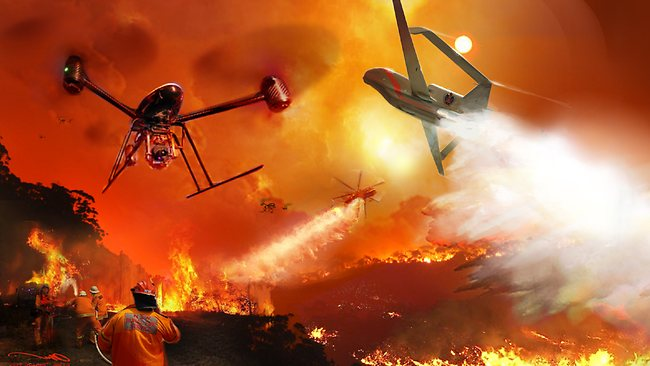
\includegraphics[width=0.7\linewidth]{ffdrones.jpg}
    \end{figure}
}

\section{Metrics}
\subsection{Risk}
\frame{\frametitle{What is Risk?}
    \begin{itemize}
        \item Risk is a representation of how dangerous or hostile
            a given area is
        \item We should minimize the frequency of data collection in areas
            or risk
        \item \emph{Examples}:
            \begin{itemize}
                \item Detection by a hostile target
                \item Damage to the vehicle due to fire
                \item Wind speeds
                \item Uncertainty of \emph{a priori} regional intelligence
            \end{itemize}

    \end{itemize}
}
\frame{\frametitle{What is Risk?}
    \begin{itemize}
        \item More formally 2D risk is defined as a function,
            $R_0: \mathbb{R} ^ 2 \rightarrow [0, 1]$
        \item Risk in 3D is the just a exponential decay of the initial risk
            but also parametrized by the altitude,
            $R: \mathbb{R} ^ 3 \rightarrow [0, 1]$
    \end{itemize}
    \begin{figure}[h!]
        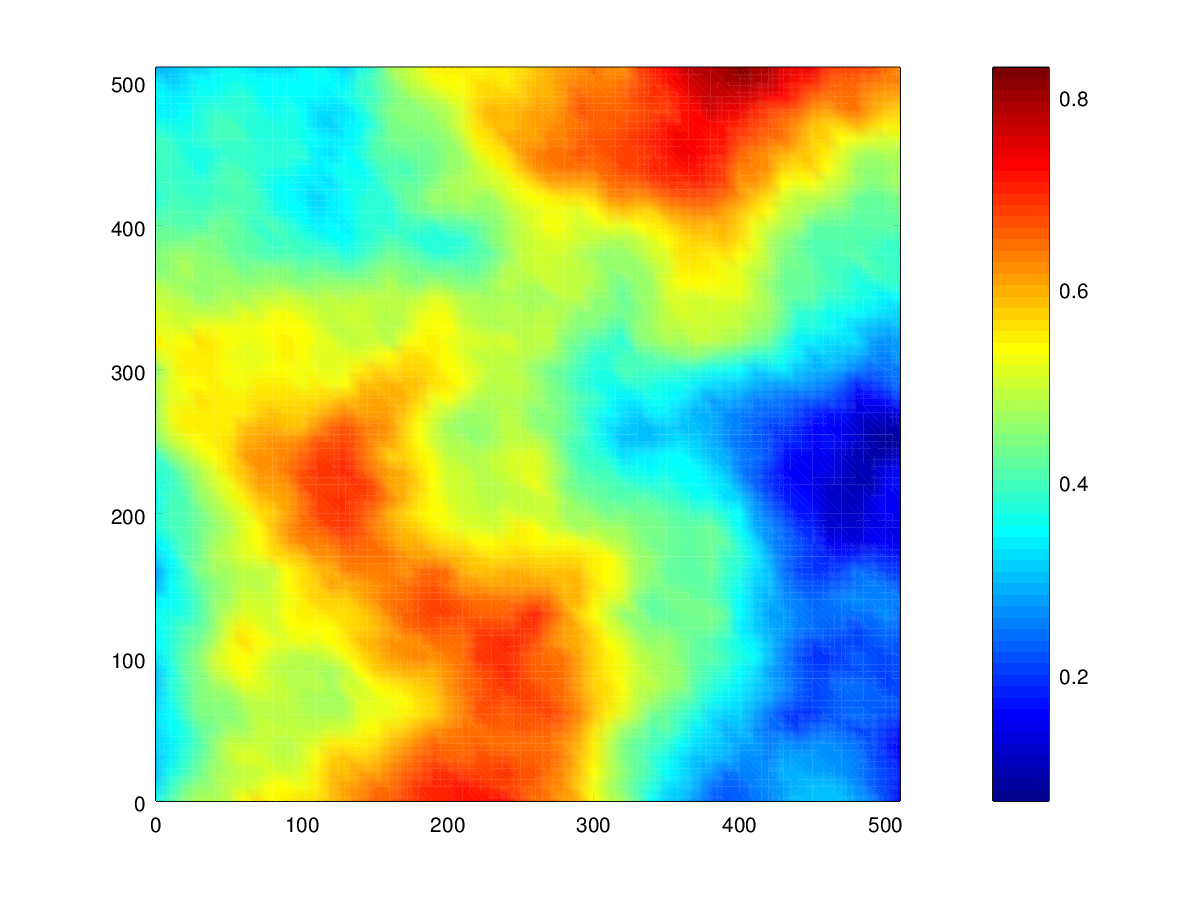
\includegraphics[width=0.6\linewidth]{risk.png}
    \end{figure}
}

\frame{\frametitle{How to Mitigate Potential Risk?}
    \begin{itemize}
        \item Minimize frequency of surveillance for regions of high risk
        \item Increase the altitude in order to maintain high absolute distance from
            a ground level risk area
        \item The policies will change depending on the type of risk
    \end{itemize}
    \begin{figure}[h!]
        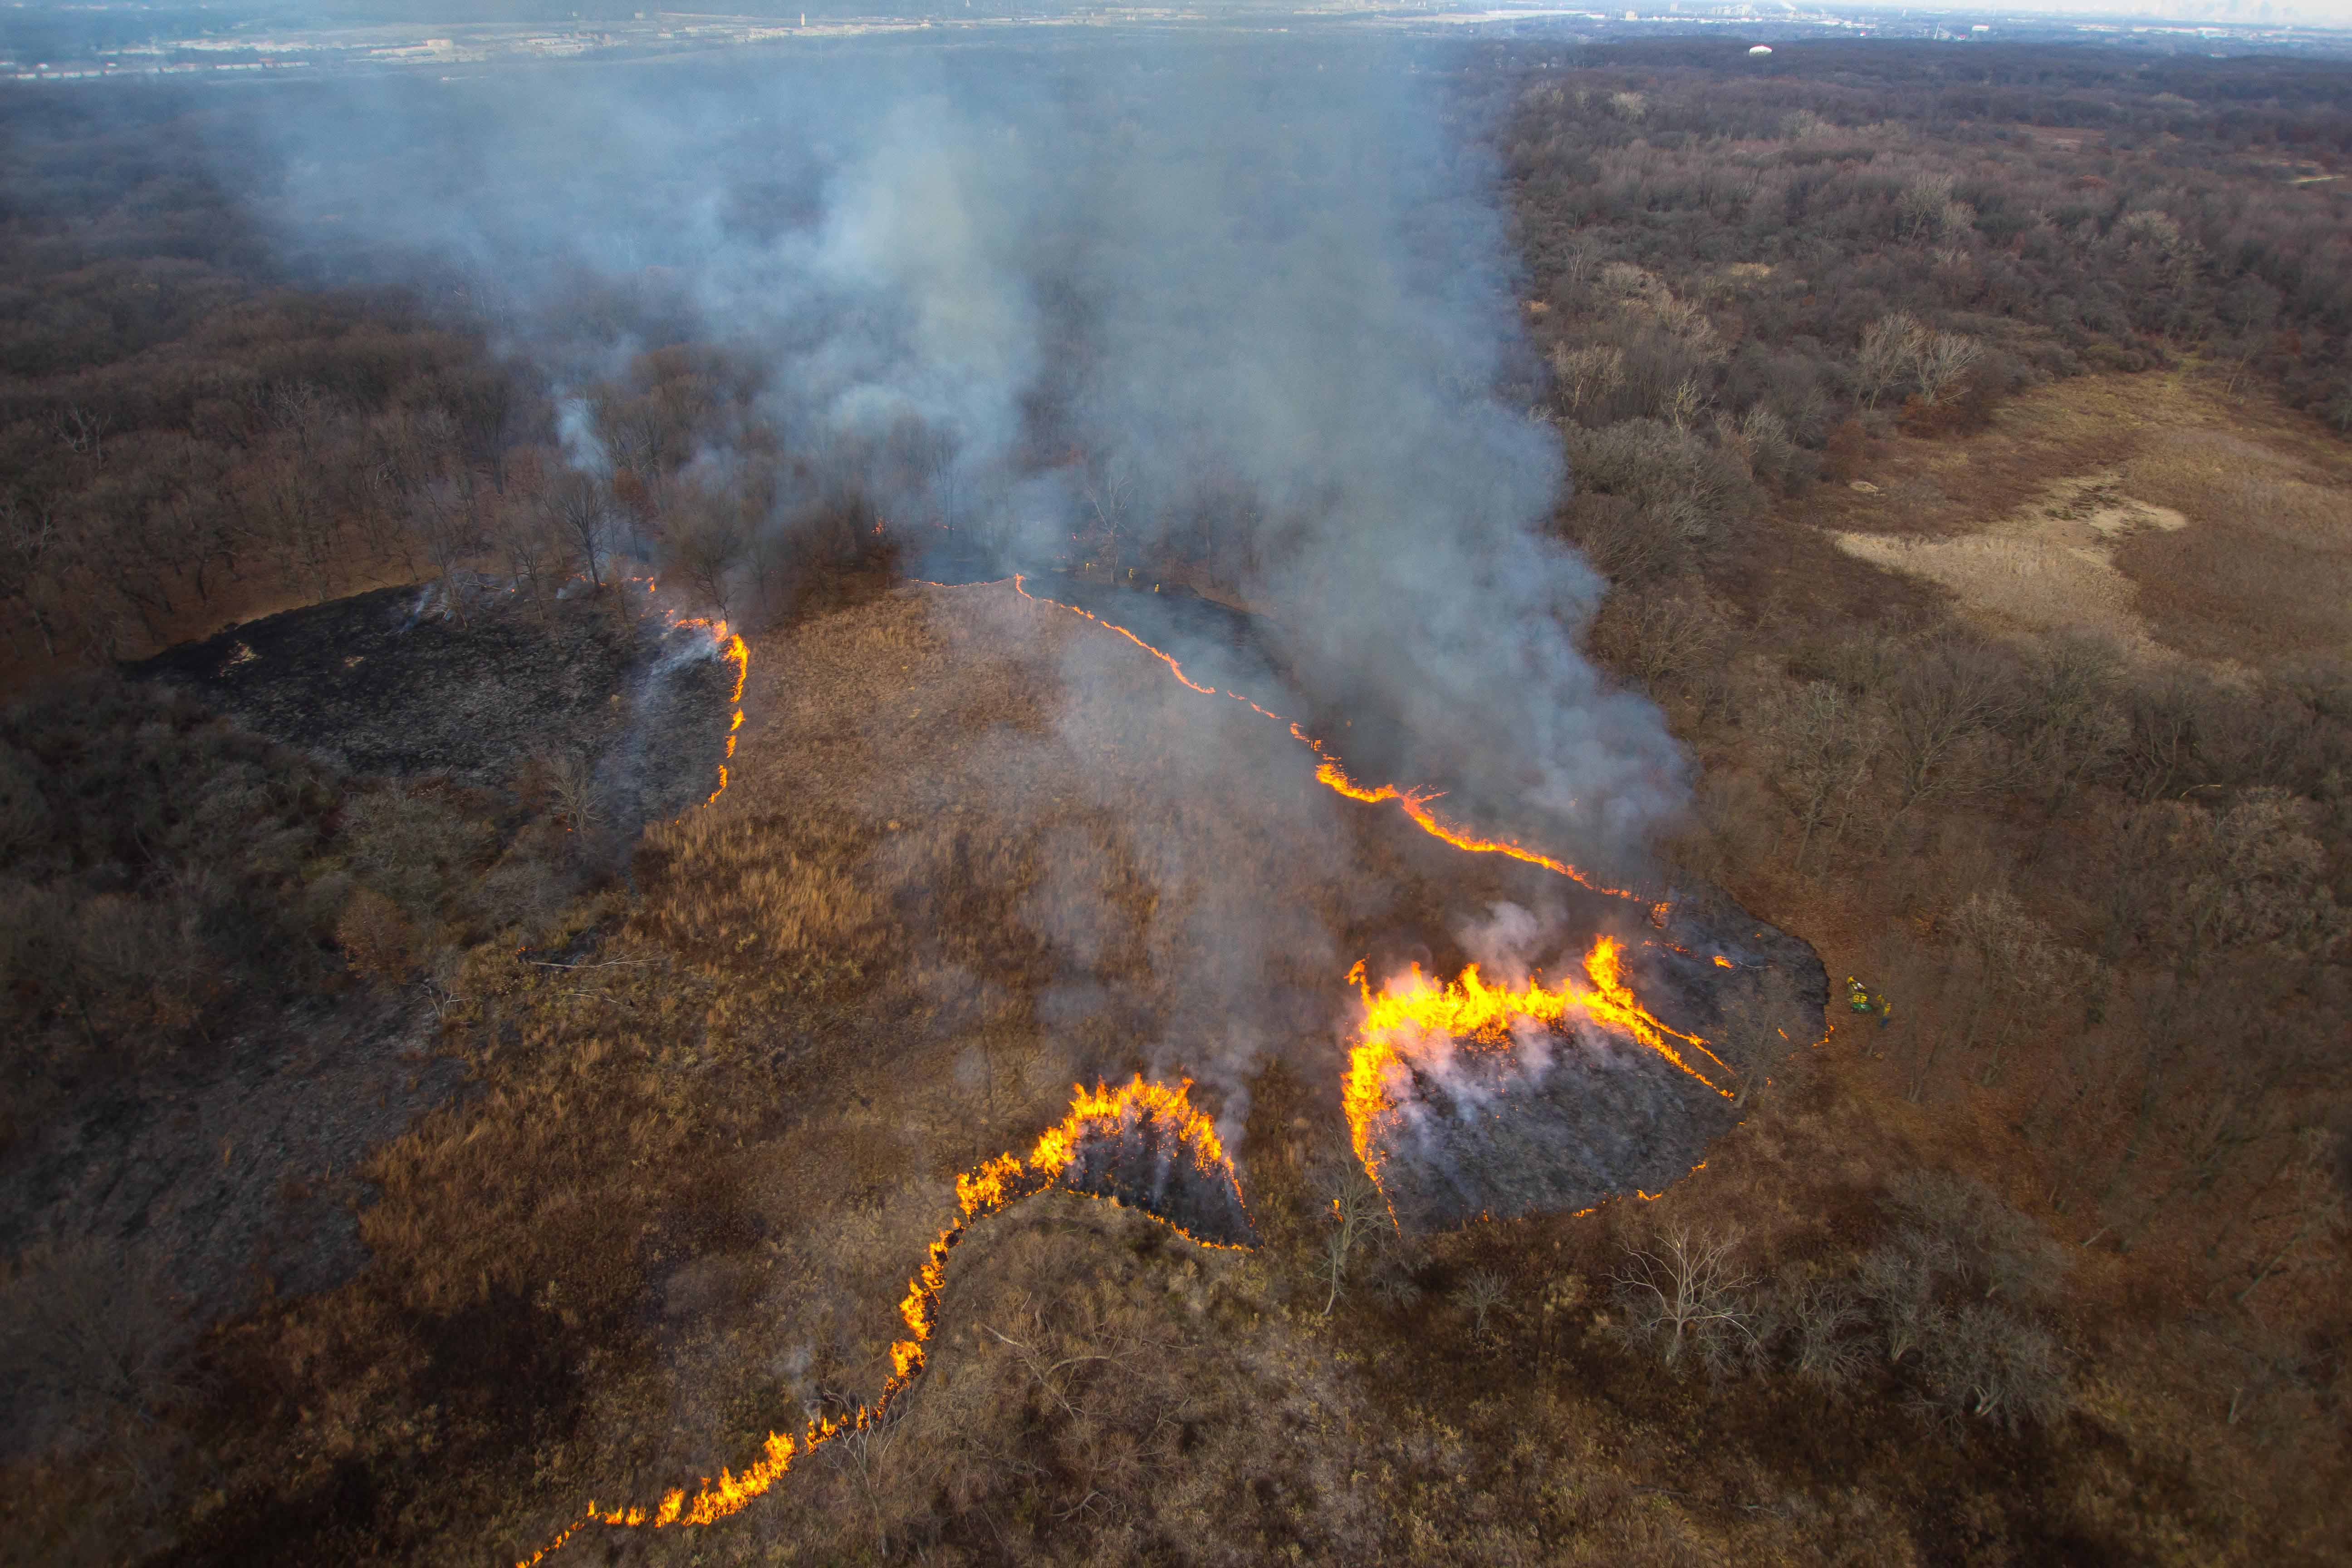
\includegraphics[width=0.6\textwidth]{fire.jpg}
    \end{figure}
}

\subsection{Sensor Quality}
\frame{\frametitle{What is Sensor Quality}
    \begin{itemize}
        \item In our experiments, the sensor quality was the quality of 
            information being retrieved from a camera
        \item Many aspects about the state of the robot affect this metric
        \item We focused on the altitude and motion blur
        \item However, different measures can be used be for sensor quality
    \end{itemize}
}

\frame{\frametitle{Motion Blur}
    \begin{itemize}
        \item Increases as the speed of the vehicle increases
        \item Can be sensed at each iteration
        \item Need to determine a optimal velocity that minimizes the
            motion blur but still does not bring the robot to a standstill
    \end{itemize}
    \begin{figure}[h!]
        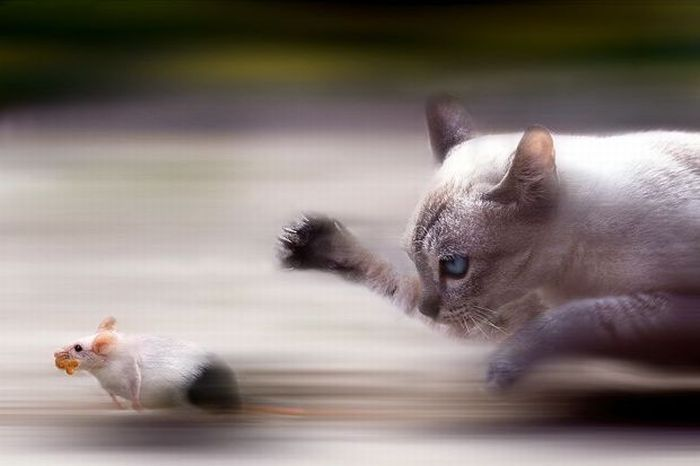
\includegraphics[width=0.5\linewidth]{cat.jpg}
    \end{figure}
}

\frame{\frametitle{Altitude}
    \begin{itemize}
        \item The altitude determines the distance away from the ground
            that images are being captured from
        \item Too high, and objects in the image are small to be recognized
        \item Too low, and objects in the image are indiscernible
    \end{itemize}
    \begin{figure}[h!]
        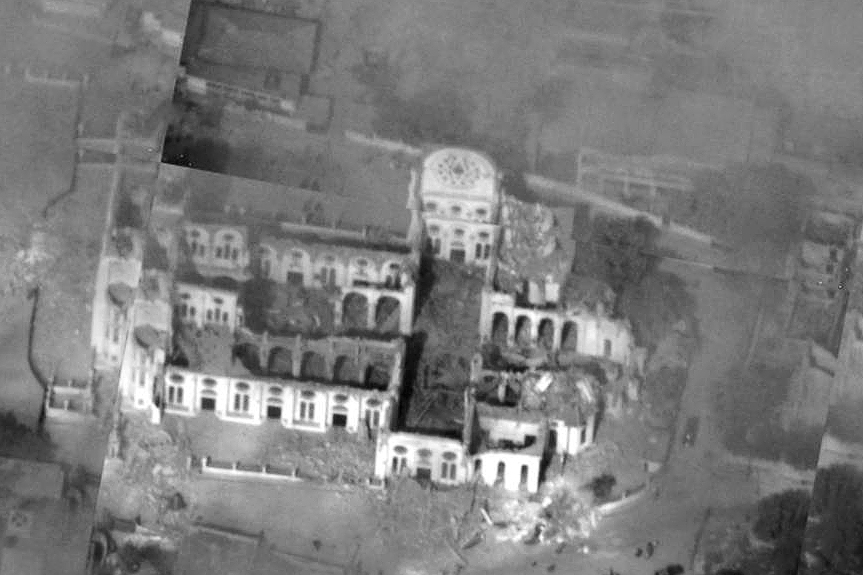
\includegraphics[width=0.5\linewidth]{drone_img.jpg}
    \end{figure}
}

\section{Motion Planning}
\subsection{Proposed Approach}
\frame{\frametitle{Proposed Approach}
    \begin{figure}
        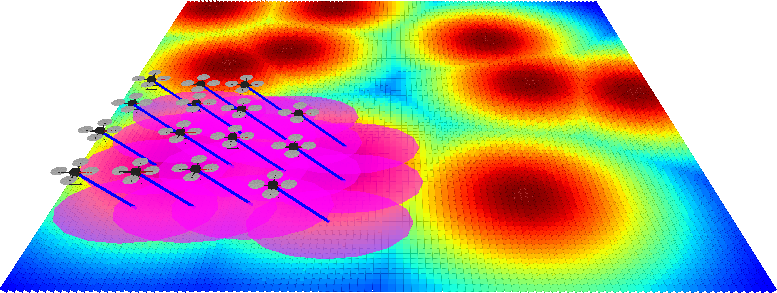
\includegraphics[width=0.49\columnwidth]{usef/rover1.png}
        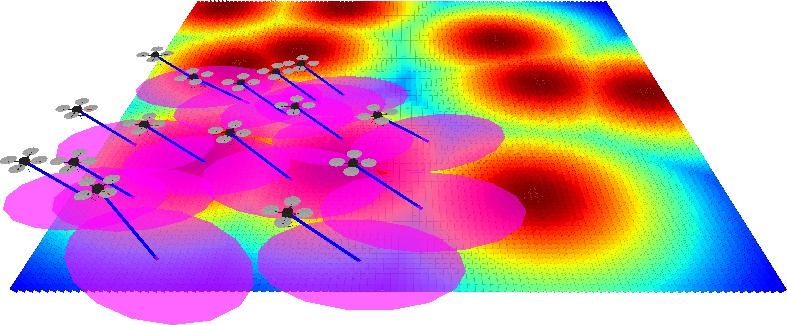
\includegraphics[width=0.49\columnwidth]{usef/rover2.png}\\
        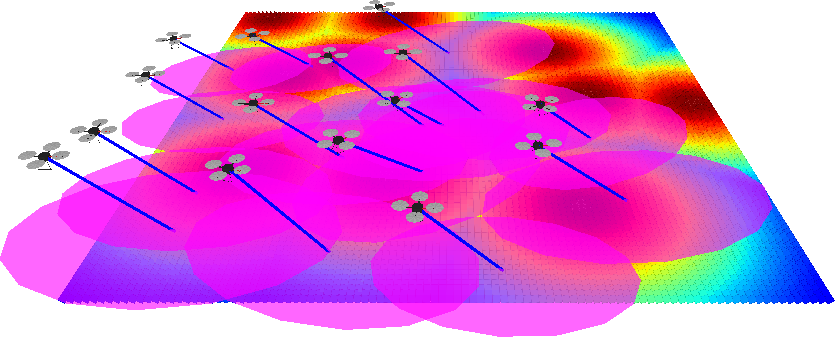
\includegraphics[width=0.49\columnwidth]{usef/rover3.png}
        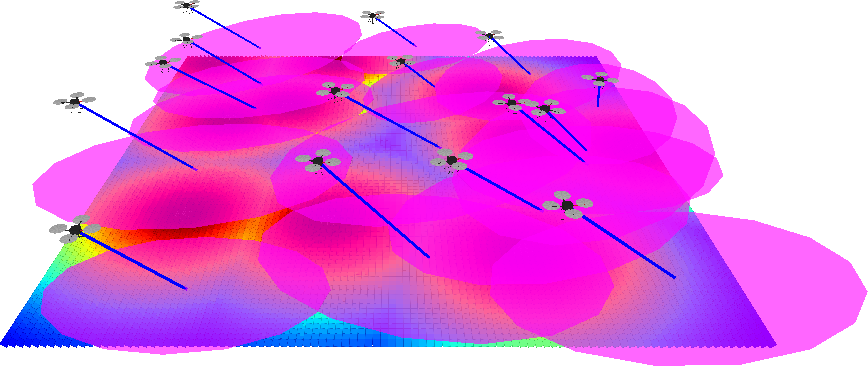
\includegraphics[width=0.49\columnwidth]{usef/rover4.png}
    \end{figure}
}

\frame{\frametitle{Proposed Approach}
    \begin{itemize}
        \item We break the planning problem into two parts
            \begin{enumerate}
                \item Plan for 2D velocity
                \item Plan for the altitude
            \end{enumerate}
        \item For 2D planning
            \begin{itemize}
                \item Move to regions of the map, $M$, that have a combination
                    largest uncertainty, $\Upsilon$, and the lowest risk, $R$
                \item Decrease the speed to minimize motion blur whilst
                    maximizing the information capture rate
            \end{itemize}
        \item For altitude planning
            \begin{itemize}
                \item Determine the altitude by maximizing the sensor quality
                    whilst minimizing the risk
            \end{itemize}
    \end{itemize}
}

\subsection{2D Planning}
\frame{\frametitle{Determining Where to Move}
    \begin{itemize}
        \item Our implementation uses a cost surface that is shared
            between the members in the swarm
        \item To determine a new heading:
            \begin{enumerate}
                \item An agent samples costs from the surface around
                    the edge of its sensor foot print,
                \item Moves in the direction of the smallest cost,
                \item And updates the uncertainty measurements in the cost
                    surface for the area that sensor foot print just covered
            \end{enumerate}
    \end{itemize}
}

\frame{\frametitle{Cost Surface \& Uncertainty}
    \begin{itemize}
        \item The cost surface, $\Gamma$, is made up of a combination of
            of the uncertainty measurements and the risk surface of the region
        \item More formally, $\Gamma(x, y) = \delta(\Upsilon(x, y), R(x, y))$
        \item Where $\delta: \mathbb{R} ^ 2 \rightarrow \mathbb{R}$ is a
            user defined function that combines the uncertainty and risk into
            one metric
    \end{itemize}
}

\frame{\frametitle{Cost Surface \& Uncertainty}
     \begin{figure}[h!]
        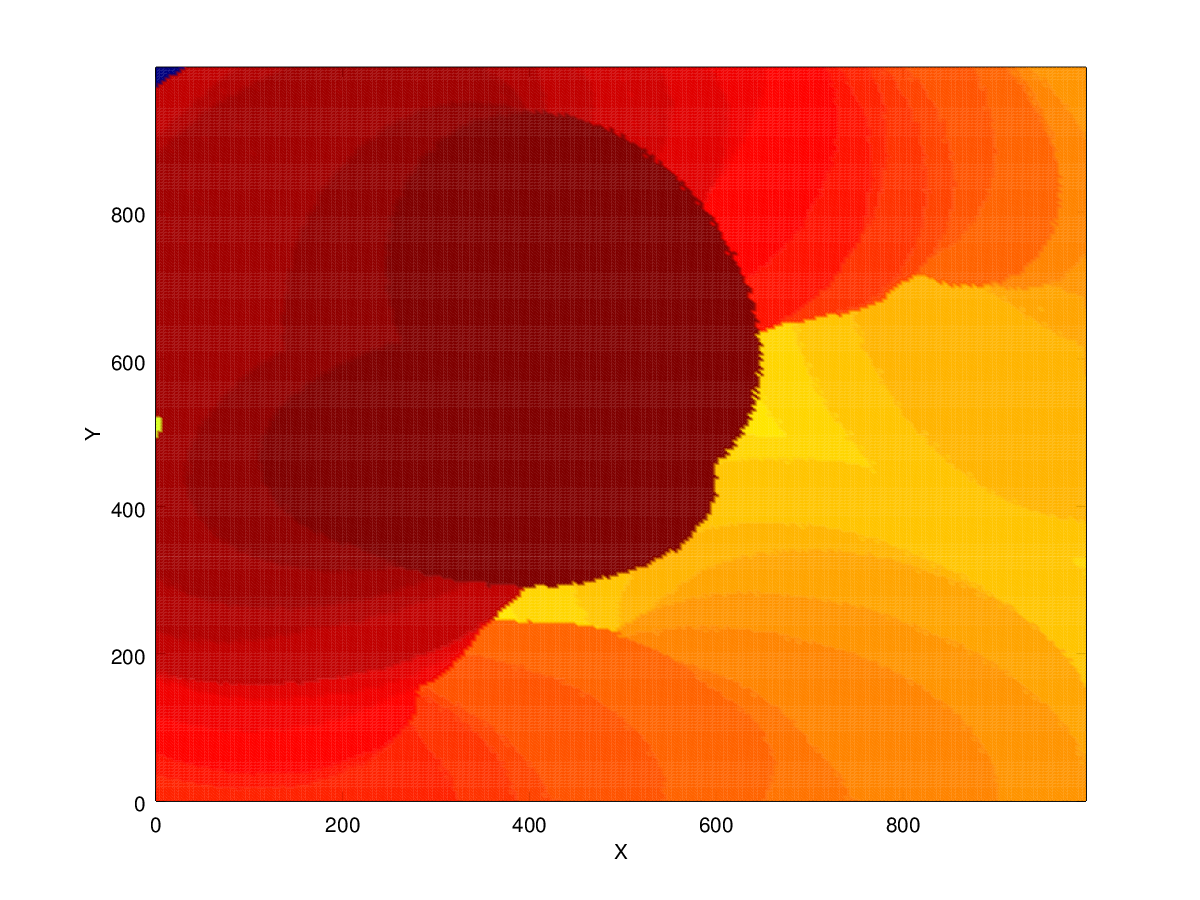
\includegraphics[width=0.8\linewidth]{usef/new_grid.png}
    \end{figure}
}

\frame{\frametitle{Determining the Speed}
    \begin{itemize}
        \item An optimal speed can be achieved by maximizing the
            information capture rate, $ICR$, whilst minimizing
            the motion blur, $MB$
        \item Formally, we maximize $ICR(v) - MB(v)$
    \end{itemize}

    \begin{figure}[h!]
        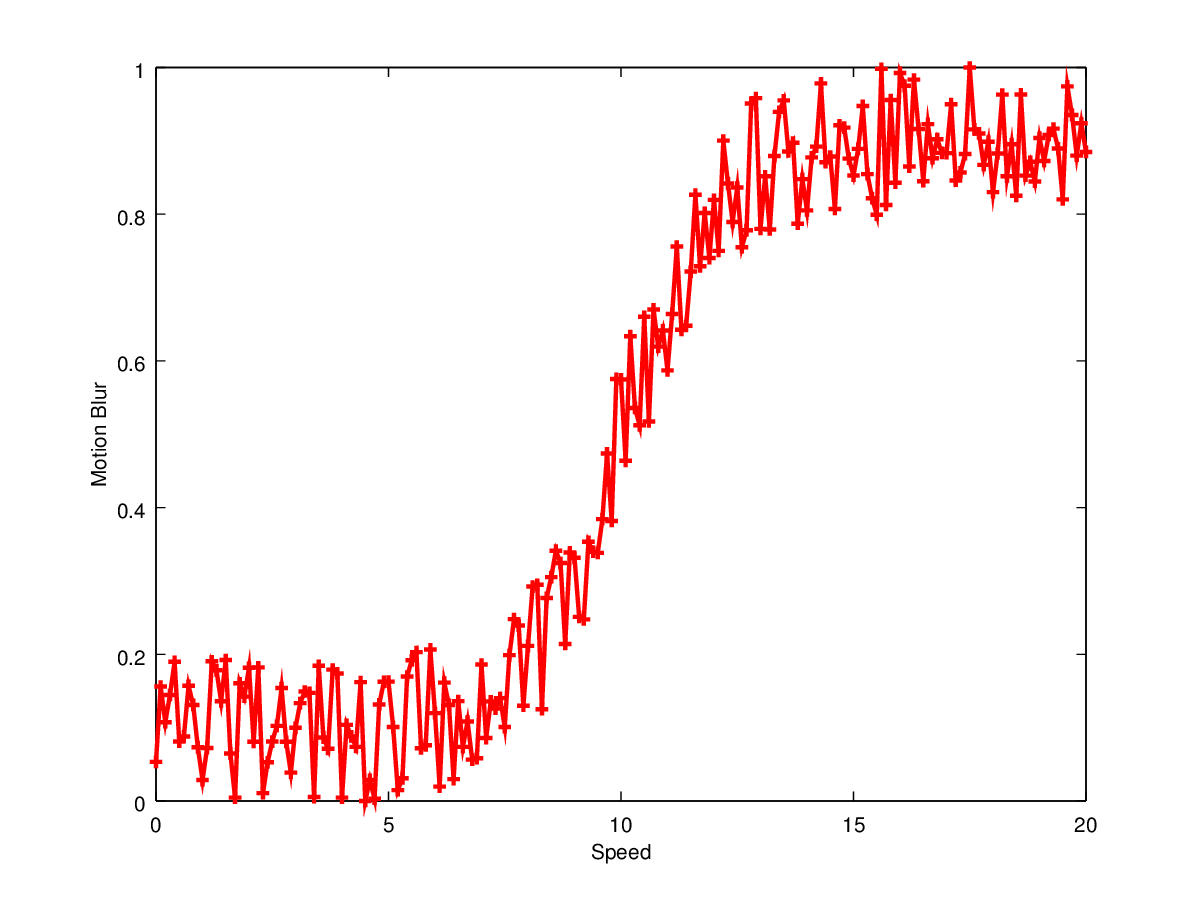
\includegraphics[width=0.5\linewidth]{sig.png}
    \end{figure}
}

\subsection{Altitude Planning}
\frame{\frametitle{Determining the Altitude}
    \begin{itemize}
        \item To determine the desired altitude, we must maximize the
            sensor quality whilst minimizing the risk with respect to $z$
        \item $Alt(x, y) = \argmax{z} SQ(z) - R(x, y, z)$
        \item This means that we are avoiding the risk by increasing the
            altitude, but are limiting the altitude by the decay in the
            sensor quality
    \end{itemize}
}

\section{Results}
\frame{\frametitle{Trajectories}
    \begin{figure}[h!]
        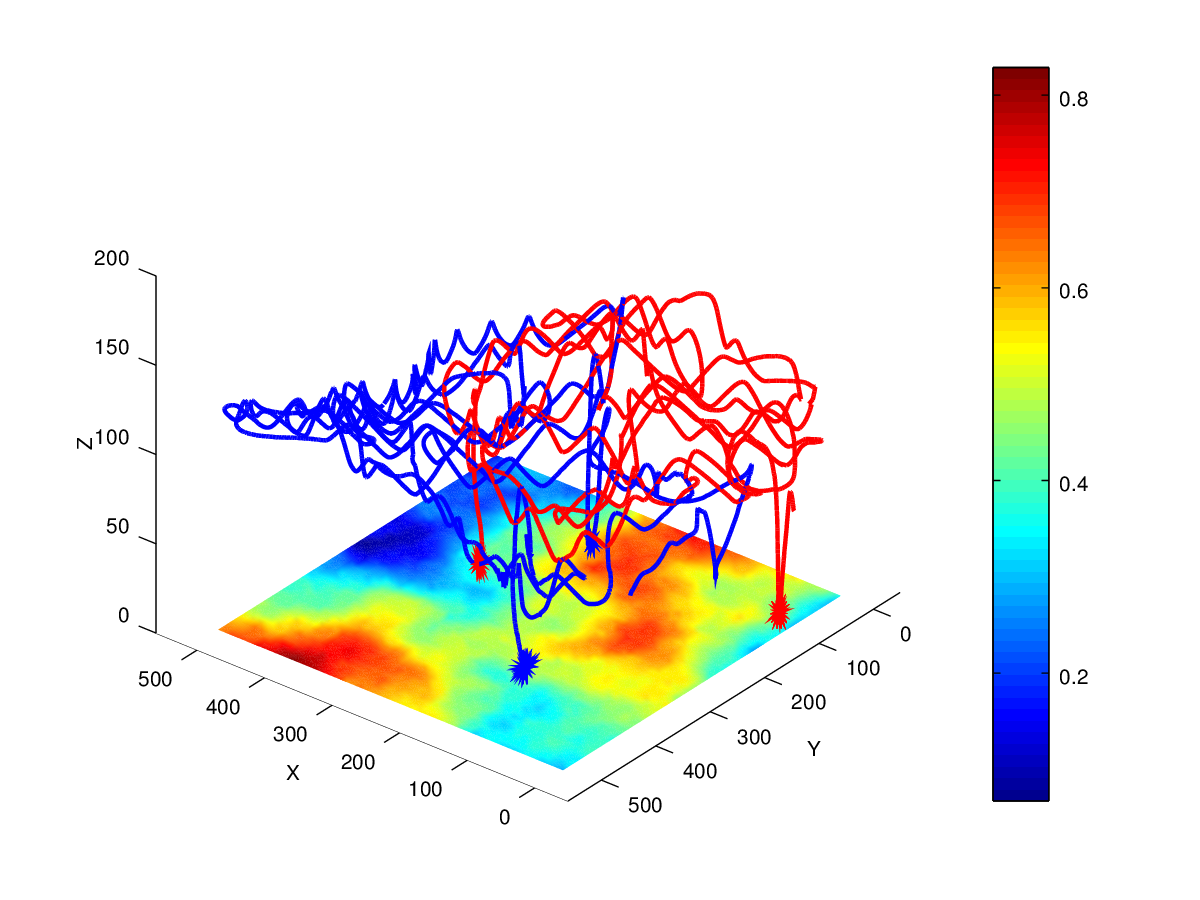
\includegraphics[width=0.8\linewidth]{trajpractical.png}
    \end{figure}
}

\frame{\frametitle{Instance Results}
    \begin{figure}
        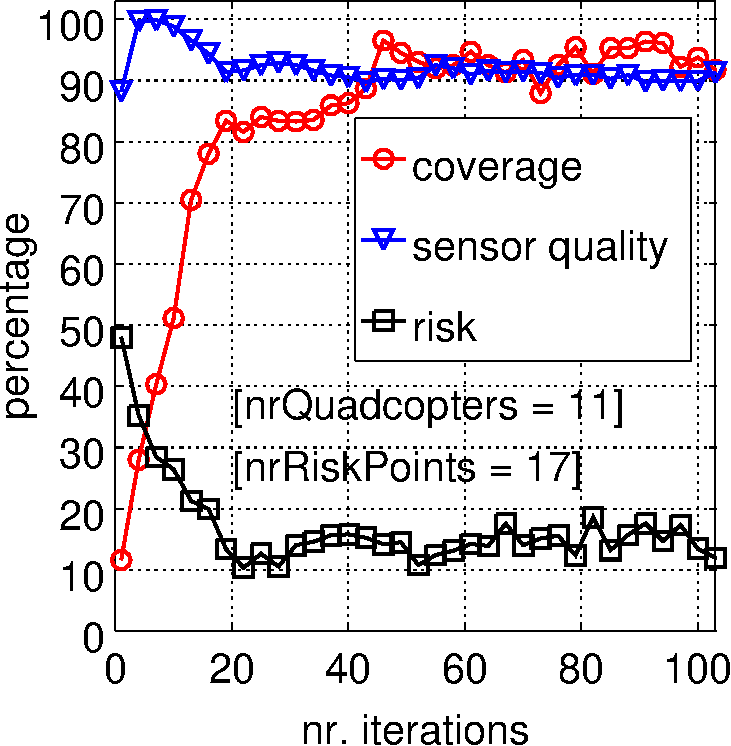
\includegraphics[width=0.4\textwidth]{usef/figResTimelineR17Q11}
        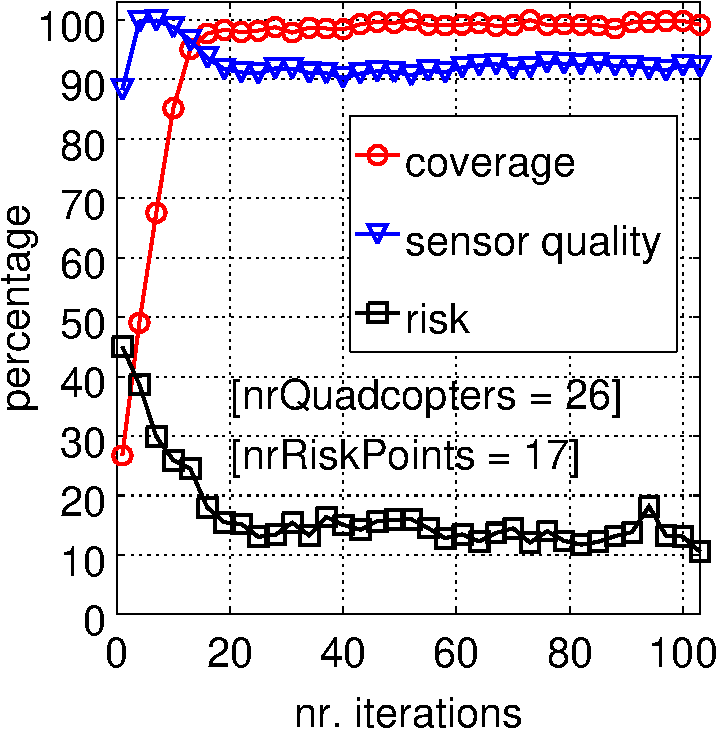
\includegraphics[width=0.4\textwidth]{usef/figResTimelineR17Q26}
    \end{figure}
}

\frame{\frametitle{Quadrotors}
    \begin{figure}
        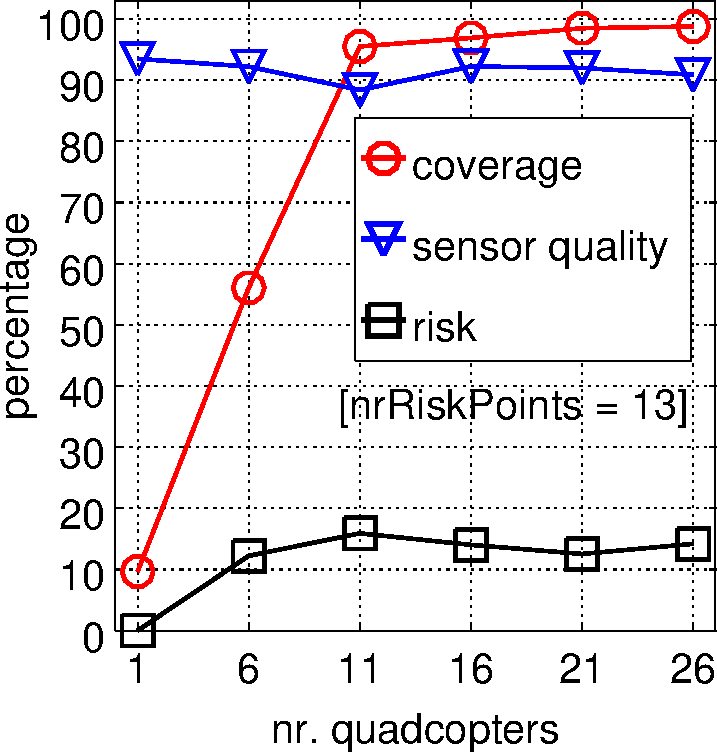
\includegraphics[width=0.32\textwidth]{usef/figResQuadsR13}
        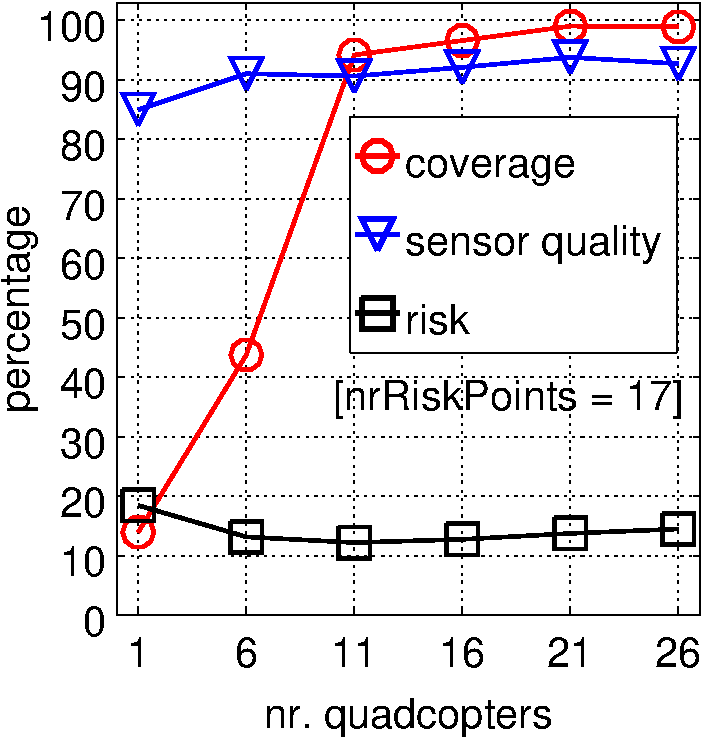
\includegraphics[width=0.32\textwidth]{usef/figResQuadsR17}
        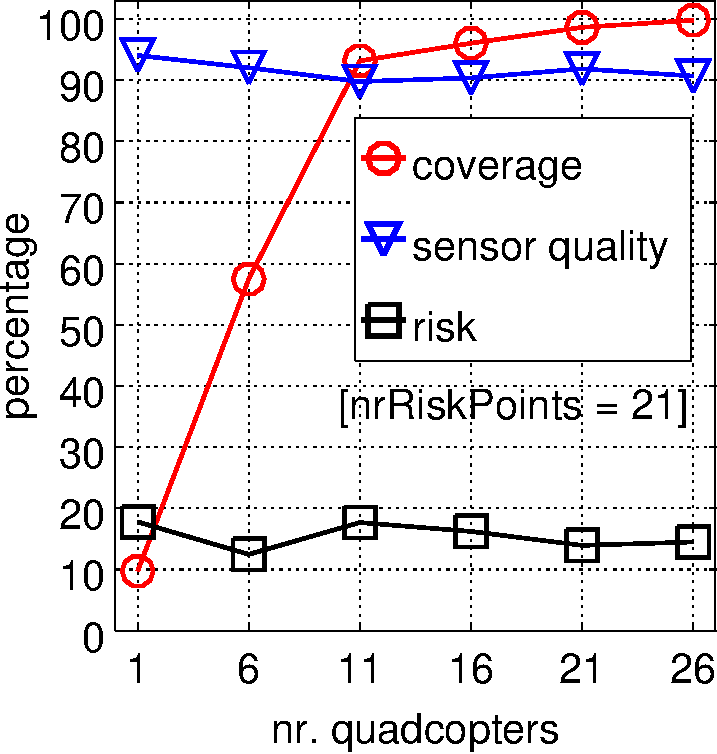
\includegraphics[width=0.32\textwidth]{usef/figResQuadsR21}
    \end{figure}
}

\frame{\frametitle{Timing}
    \begin{figure}
        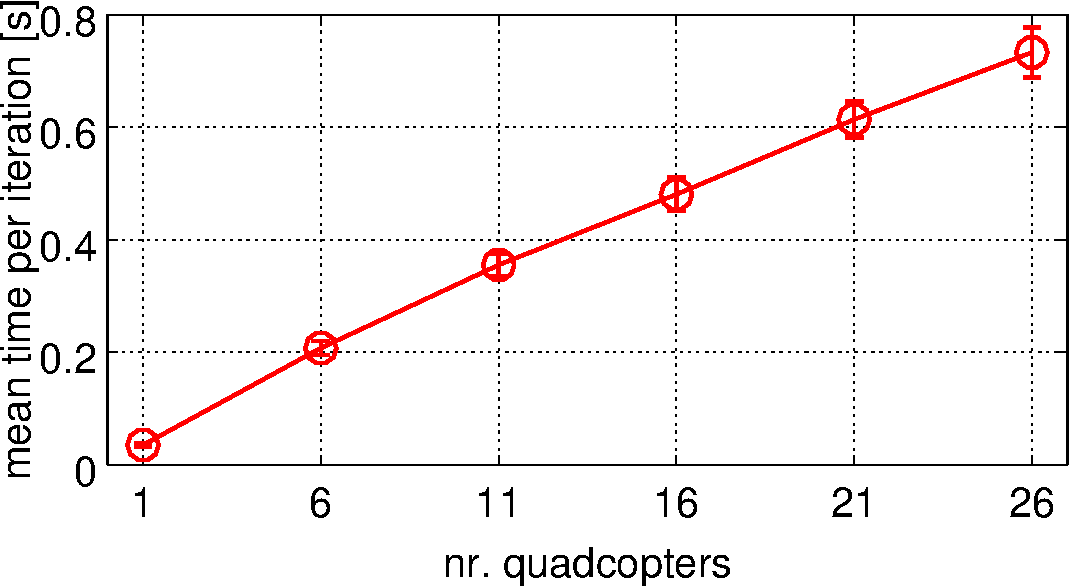
\includegraphics[width=0.8\columnwidth]{figResTimePerIter}
    \end{figure}
}

\section{Conclusions}
\frame{\frametitle{Conclusions}
    \begin{itemize}
        \item The proposed approach minimizes the measured risk whilst
            maximizing the sensor quality by varying the altitude and
            reducing the frequency of coverage for risky regions
        \item The algorithmic time increases linearly with respect to the
            number of quadrotors
        \item The quadrotors are quick to reach area coverage convergence
    \end{itemize}
}

\end{document}

